\documentclass[twoside]{book}

% Packages required by doxygen
\usepackage{fixltx2e}
\usepackage{calc}
\usepackage{doxygen}
\usepackage{graphicx}
\usepackage[utf8]{inputenc}
\usepackage{makeidx}
\usepackage{multicol}
\usepackage{multirow}
\PassOptionsToPackage{warn}{textcomp}
\usepackage{textcomp}
\usepackage[nointegrals]{wasysym}
\usepackage[table]{xcolor}
\usepackage{ifpdf,ifxetex}

% Font selection
\usepackage[T1]{fontenc}
\usepackage[scaled=.90]{helvet}
\usepackage{courier}
\usepackage{amssymb}
\usepackage{sectsty}
\renewcommand{\familydefault}{\sfdefault}
\allsectionsfont{%
  \fontseries{bc}\selectfont%
  \color{darkgray}%
}
\renewcommand{\DoxyLabelFont}{%
  \fontseries{bc}\selectfont%
  \color{darkgray}%
}
\newcommand{\+}{\discretionary{\mbox{\scriptsize$\hookleftarrow$}}{}{}}

% Page & text layout
\usepackage{geometry}
\geometry{%
  a4paper,%
  top=2.5cm,%
  bottom=2.5cm,%
  left=2.5cm,%
  right=2.5cm%
}
\tolerance=750
\hfuzz=15pt
\hbadness=750
\setlength{\emergencystretch}{15pt}
\setlength{\parindent}{0cm}
\setlength{\parskip}{3ex plus 2ex minus 2ex}
\makeatletter
\renewcommand{\paragraph}{%
  \@startsection{paragraph}{4}{0ex}{-1.0ex}{1.0ex}{%
    \normalfont\normalsize\bfseries\SS@parafont%
  }%
}
\renewcommand{\subparagraph}{%
  \@startsection{subparagraph}{5}{0ex}{-1.0ex}{1.0ex}{%
    \normalfont\normalsize\bfseries\SS@subparafont%
  }%
}
\makeatother

% Headers & footers
\usepackage{fancyhdr}
\pagestyle{fancyplain}
\fancyhead[LE]{\fancyplain{}{\bfseries\thepage}}
\fancyhead[CE]{\fancyplain{}{}}
\fancyhead[RE]{\fancyplain{}{\bfseries\leftmark}}
\fancyhead[LO]{\fancyplain{}{\bfseries\rightmark}}
\fancyhead[CO]{\fancyplain{}{}}
\fancyhead[RO]{\fancyplain{}{\bfseries\thepage}}
\fancyfoot[LE]{\fancyplain{}{}}
\fancyfoot[CE]{\fancyplain{}{}}
\fancyfoot[RE]{\fancyplain{}{\bfseries\scriptsize Generated by Doxygen }}
\fancyfoot[LO]{\fancyplain{}{\bfseries\scriptsize Generated by Doxygen }}
\fancyfoot[CO]{\fancyplain{}{}}
\fancyfoot[RO]{\fancyplain{}{}}
\renewcommand{\footrulewidth}{0.4pt}
\renewcommand{\chaptermark}[1]{%
  \markboth{#1}{}%
}
\renewcommand{\sectionmark}[1]{%
  \markright{\thesection\ #1}%
}

% Indices & bibliography
\usepackage{natbib}
\usepackage[titles]{tocloft}
\setcounter{tocdepth}{3}
\setcounter{secnumdepth}{5}
\makeindex

% Hyperlinks (required, but should be loaded last)
\ifpdf
  \usepackage[pdftex,pagebackref=true]{hyperref}
\else
  \ifxetex
    \usepackage[pagebackref=true]{hyperref}
  \else
    \usepackage[ps2pdf,pagebackref=true]{hyperref}
  \fi
\fi
\ifpdf
  \DeclareUnicodeCharacter{207B}{${}^{-}$}% Superscript minus
  \DeclareUnicodeCharacter{C2B2}{${}^{2}$}% Superscript two
  \DeclareUnicodeCharacter{C2B3}{${}^{3}$}% Superscript three
\else
  \catcode`\⁻=13% Superscript minus
  \def⁻{${}^{-}$}
  \catcode`\²=13% Superscript two
  \def²{${}^{2}$}
  \catcode`\³=13% Superscript three
  \def³{${}^{3}$}
\fi

\hypersetup{%
  colorlinks=true,%
  linkcolor=blue,%
  citecolor=blue,%
  unicode%
}

% Custom commands
\newcommand{\clearemptydoublepage}{%
  \newpage{\pagestyle{empty}\cleardoublepage}%
}

\usepackage{caption}
\captionsetup{labelsep=space,justification=centering,font={bf},singlelinecheck=off,skip=4pt,position=top}

\renewcommand{\numberline}[1]{#1~}
%===== C O N T E N T S =====

\begin{document}

% Titlepage & ToC
\hypersetup{pageanchor=false,
             bookmarksnumbered=true,
             pdfencoding=unicode
            }
\pagenumbering{alph}
\begin{titlepage}
\vspace*{7cm}
\begin{center}%
{\Large moebinv-\/gui }\\
\vspace*{1cm}
{\large Generated by Doxygen 1.8.15}\\
\end{center}
\end{titlepage}
\clearemptydoublepage
\pagenumbering{roman}
\tableofcontents
\clearemptydoublepage
\pagenumbering{arabic}
\hypersetup{pageanchor=true}

%--- Begin generated contents ---
\chapter{moebinv-\/gui}
\label{md___users_lukehutton__one_drive_-__university_of__leeds__university__computer__science__internship_moebinv-gui__r_e_a_d_m_e}
\Hypertarget{md___users_lukehutton__one_drive_-__university_of__leeds__university__computer__science__internship_moebinv-gui__r_e_a_d_m_e}
This application provides a G\+UI for the moebinv package.

\subsection*{Table of Contents}


\begin{DoxyItemize}
\item \href{#introduction}{\tt Introduction}
\item \href{#installation}{\tt Installation}
\item \href{#usage}{\tt Usage}
\end{DoxyItemize}

\subsection*{Introduction}

The moebinv library allows for manipulations in non euclidean geometry. This application is a gui for use with the moebinv library.

\subsection*{Installation}

Prerequisites\+:
\begin{DoxyItemize}
\item C\+LN
\item Gi\+NaC
\item moebinv
\end{DoxyItemize}

\subsection*{Usage}

Replace the contents of {\ttfamily R\+E\+A\+D\+M\+E.\+md} with your project\textquotesingle{}s\+:


\begin{DoxyItemize}
\item Name
\item Description
\item Installation instructions
\item Usage instructions
\item Support instructions
\item Contributing instructions
\end{DoxyItemize}

Feel free to remove any sections that aren\textquotesingle{}t applicable to your project. 
\chapter{Hierarchical Index}
\section{Class Hierarchy}
This inheritance list is sorted roughly, but not completely, alphabetically\+:\begin{DoxyCompactList}
\item \contentsline{section}{cycle\+Data}{\pageref{structcycle_data}}{}
\item \contentsline{section}{cycle\+Style\+Data}{\pageref{structcycle_style_data}}{}
\item \contentsline{section}{labels}{\pageref{classlabels}}{}
\item Q\+Action\+Group\begin{DoxyCompactList}
\item \contentsline{section}{menu\+Rel\+Action\+Group}{\pageref{classmenu_rel_action_group}}{}
\end{DoxyCompactList}
\item Q\+Dialog\begin{DoxyCompactList}
\item \contentsline{section}{define\+Cycle\+Dialog}{\pageref{classdefine_cycle_dialog}}{}
\item \contentsline{section}{help\+Dialog}{\pageref{classhelp_dialog}}{}
\item \contentsline{section}{matrix4dialog}{\pageref{classmatrix4dialog}}{}
\item \contentsline{section}{matrix8dialog}{\pageref{classmatrix8dialog}}{}
\item \contentsline{section}{properties\+Dialog}{\pageref{classproperties_dialog}}{}
\item \contentsline{section}{settings\+Dialog}{\pageref{classsettings_dialog}}{}
\end{DoxyCompactList}
\item Q\+Dock\+Widget\begin{DoxyCompactList}
\item \contentsline{section}{dock\+Widget}{\pageref{classdock_widget}}{}
\end{DoxyCompactList}
\item Q\+Graphics\+Item\begin{DoxyCompactList}
\item \contentsline{section}{circle}{\pageref{classcircle}}{}
\item \contentsline{section}{graphic\+Cycle}{\pageref{classgraphic_cycle}}{}
\item \contentsline{section}{line}{\pageref{classline}}{}
\item \contentsline{section}{point}{\pageref{classpoint}}{}
\end{DoxyCompactList}
\item Q\+Graphics\+Scene\begin{DoxyCompactList}
\item \contentsline{section}{graphics\+Scene}{\pageref{classgraphics_scene}}{}
\end{DoxyCompactList}
\item Q\+Graphics\+View\begin{DoxyCompactList}
\item \contentsline{section}{view}{\pageref{classview}}{}
\end{DoxyCompactList}
\item Q\+Main\+Window\begin{DoxyCompactList}
\item \contentsline{section}{Main\+Window}{\pageref{class_main_window}}{}
\end{DoxyCompactList}
\item Q\+Menu\begin{DoxyCompactList}
\item \contentsline{section}{cycle\+Context\+Menu}{\pageref{classcycle_context_menu}}{}
\end{DoxyCompactList}
\item Q\+Object\begin{DoxyCompactList}
\item \contentsline{section}{circle}{\pageref{classcircle}}{}
\item \contentsline{section}{figure\+Undo\+Command}{\pageref{classfigure_undo_command}}{}
\item \contentsline{section}{graphic\+Cycle}{\pageref{classgraphic_cycle}}{}
\item \contentsline{section}{line}{\pageref{classline}}{}
\item \contentsline{section}{menu\+Rel\+Action}{\pageref{classmenu_rel_action}}{}
\item \contentsline{section}{point}{\pageref{classpoint}}{}
\end{DoxyCompactList}
\item Q\+Standard\+Item\+Model\begin{DoxyCompactList}
\item \contentsline{section}{tree\+Model}{\pageref{classtree_model}}{}
\end{DoxyCompactList}
\item Q\+Text\+Browser\begin{DoxyCompactList}
\item \contentsline{section}{help\+Browser}{\pageref{classhelp_browser}}{}
\end{DoxyCompactList}
\item Q\+Undo\+Command\begin{DoxyCompactList}
\item \contentsline{section}{figure\+Undo\+Command}{\pageref{classfigure_undo_command}}{}
\end{DoxyCompactList}
\end{DoxyCompactList}

\chapter{Class Index}
\section{Class List}
Here are the classes, structs, unions and interfaces with brief descriptions\+:\begin{DoxyCompactList}
\item\contentsline{section}{\mbox{\hyperlink{class_main_window}{Main\+Window}} }{\pageref{class_main_window}}{}
\end{DoxyCompactList}

\chapter{Class Documentation}
\hypertarget{classcircle}{}\section{circle Class Reference}
\label{classcircle}\index{circle@{circle}}
Inheritance diagram for circle\+:\begin{figure}[H]
\begin{center}
\leavevmode
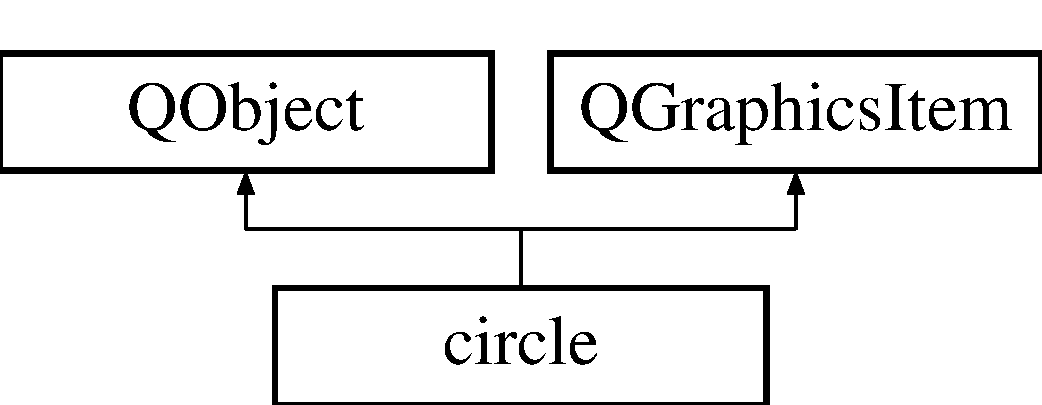
\includegraphics[height=2.000000cm]{classcircle}
\end{center}
\end{figure}
\subsection*{Public Member Functions}
\begin{DoxyCompactItemize}
\item 
\mbox{\hyperlink{classcircle_abfd721dc65145023cf14739adacc81a8}{circle}} (\mbox{\hyperlink{classgraphic_cycle}{graphic\+Cycle}} $\ast$parent, struct \mbox{\hyperlink{structcycle_data}{cycle\+Data}} data)
\begin{DoxyCompactList}\small\item\em circle\+::line Create a new circle. \end{DoxyCompactList}\item 
void \mbox{\hyperlink{classcircle_a2d9af8e86fb3605c736689a2e2566d26}{paint}} (Q\+Painter $\ast$painter, const Q\+Style\+Option\+Graphics\+Item $\ast$option, Q\+Widget $\ast$widget)
\begin{DoxyCompactList}\small\item\em \mbox{\hyperlink{classcircle_a2d9af8e86fb3605c736689a2e2566d26}{circle\+::paint}} Paint the circle on the scene. \end{DoxyCompactList}\item 
Q\+RectF \mbox{\hyperlink{classcircle_ab9d2059829ac8f0420c7e711caeb61c7}{bounding\+Rect}} () const
\begin{DoxyCompactList}\small\item\em \mbox{\hyperlink{classcircle_ab9d2059829ac8f0420c7e711caeb61c7}{circle\+::bounding\+Rect}} Define the bounding rect. \end{DoxyCompactList}\item 
Q\+Painter\+Path \mbox{\hyperlink{classcircle_a198cbcea745bd311fe91c2a23def746c}{shape}} () const
\begin{DoxyCompactList}\small\item\em \mbox{\hyperlink{classcircle_a198cbcea745bd311fe91c2a23def746c}{circle\+::shape}} Define the clipping mask of the object \end{DoxyCompactList}\end{DoxyCompactItemize}


\subsection{Constructor \& Destructor Documentation}
\mbox{\Hypertarget{classcircle_abfd721dc65145023cf14739adacc81a8}\label{classcircle_abfd721dc65145023cf14739adacc81a8}} 
\index{circle@{circle}!circle@{circle}}
\index{circle@{circle}!circle@{circle}}
\subsubsection{\texorpdfstring{circle()}{circle()}}
{\footnotesize\ttfamily circle\+::circle (\begin{DoxyParamCaption}\item[{\mbox{\hyperlink{classgraphic_cycle}{graphic\+Cycle}} $\ast$}]{parent,  }\item[{struct \mbox{\hyperlink{structcycle_data}{cycle\+Data}}}]{data }\end{DoxyParamCaption})}



circle\+::line Create a new circle. 


\begin{DoxyParams}{Parameters}
{\em struct} & \mbox{\hyperlink{structcycle_data}{cycle\+Data}} data Contains the data needed to draw the circle.\\
\hline
\end{DoxyParams}
Construct a new line on the scene and assign it to the parent \mbox{\hyperlink{classgraphic_cycle}{graphic\+Cycle}}. 

\subsection{Member Function Documentation}
\mbox{\Hypertarget{classcircle_ab9d2059829ac8f0420c7e711caeb61c7}\label{classcircle_ab9d2059829ac8f0420c7e711caeb61c7}} 
\index{circle@{circle}!bounding\+Rect@{bounding\+Rect}}
\index{bounding\+Rect@{bounding\+Rect}!circle@{circle}}
\subsubsection{\texorpdfstring{bounding\+Rect()}{boundingRect()}}
{\footnotesize\ttfamily Q\+RectF circle\+::bounding\+Rect (\begin{DoxyParamCaption}{ }\end{DoxyParamCaption}) const}



\mbox{\hyperlink{classcircle_ab9d2059829ac8f0420c7e711caeb61c7}{circle\+::bounding\+Rect}} Define the bounding rect. 

\begin{DoxyReturn}{Returns}
Q\+RectF
\end{DoxyReturn}
Define the box the object is drawn within on the scene. \mbox{\Hypertarget{classcircle_a2d9af8e86fb3605c736689a2e2566d26}\label{classcircle_a2d9af8e86fb3605c736689a2e2566d26}} 
\index{circle@{circle}!paint@{paint}}
\index{paint@{paint}!circle@{circle}}
\subsubsection{\texorpdfstring{paint()}{paint()}}
{\footnotesize\ttfamily void circle\+::paint (\begin{DoxyParamCaption}\item[{Q\+Painter $\ast$}]{painter,  }\item[{const Q\+Style\+Option\+Graphics\+Item $\ast$}]{option,  }\item[{Q\+Widget $\ast$}]{widget }\end{DoxyParamCaption})}



\mbox{\hyperlink{classcircle_a2d9af8e86fb3605c736689a2e2566d26}{circle\+::paint}} Paint the circle on the scene. 


\begin{DoxyParams}{Parameters}
{\em painter} & Q\+Painter object. \\
\hline
{\em option} & \\
\hline
{\em widget} & This function paints the point on the scene given various parameters (such as x and y). The point is drawn differently dependent on the drawing metric in use. \\
\hline
\end{DoxyParams}
\mbox{\Hypertarget{classcircle_a198cbcea745bd311fe91c2a23def746c}\label{classcircle_a198cbcea745bd311fe91c2a23def746c}} 
\index{circle@{circle}!shape@{shape}}
\index{shape@{shape}!circle@{circle}}
\subsubsection{\texorpdfstring{shape()}{shape()}}
{\footnotesize\ttfamily Q\+Painter\+Path circle\+::shape (\begin{DoxyParamCaption}{ }\end{DoxyParamCaption}) const}



\mbox{\hyperlink{classcircle_a198cbcea745bd311fe91c2a23def746c}{circle\+::shape}} Define the clipping mask of the object 

\begin{DoxyReturn}{Returns}
Q\+Painter\+Path
\end{DoxyReturn}
Defines the area in which the shape actually exists. 

The documentation for this class was generated from the following files\+:\begin{DoxyCompactItemize}
\item 
/\+Users/lukehutton/\+One\+Drive -\/ University of Leeds/\+University/\+Computer Science/\+Internship/moebinv-\/gui/include/circle.\+h\item 
/\+Users/lukehutton/\+One\+Drive -\/ University of Leeds/\+University/\+Computer Science/\+Internship/moebinv-\/gui/src/circle.\+cpp\end{DoxyCompactItemize}

\hypertarget{class_main_window}{}\section{Main\+Window Class Reference}
\label{class_main_window}\index{Main\+Window@{Main\+Window}}


The \mbox{\hyperlink{class_main_window}{Main\+Window}} class.  




{\ttfamily \#include $<$mainwindow.\+h$>$}

Inheritance diagram for Main\+Window\+:\begin{figure}[H]
\begin{center}
\leavevmode
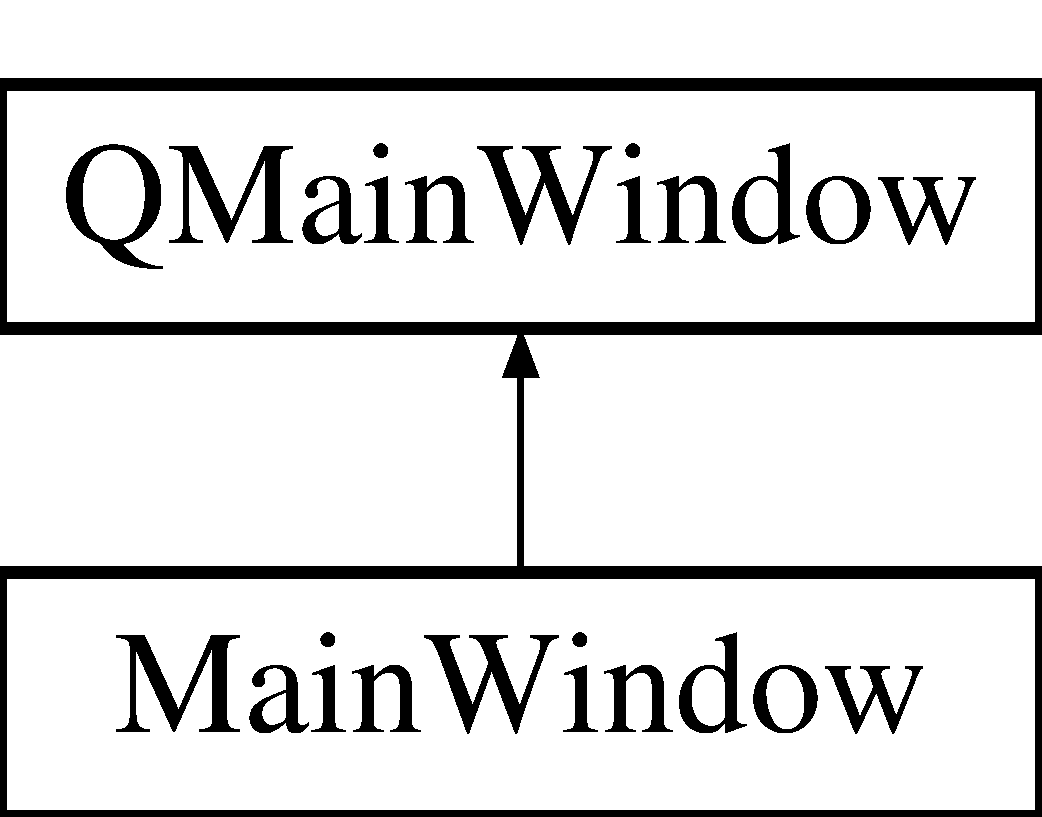
\includegraphics[height=2.000000cm]{class_main_window}
\end{center}
\end{figure}
\subsection*{Signals}
\begin{DoxyCompactItemize}
\item 
\mbox{\Hypertarget{class_main_window_a46ebd786b1aeb0ef026f0a3f32dd9f3d}\label{class_main_window_a46ebd786b1aeb0ef026f0a3f32dd9f3d}} 
void {\bfseries reset\+Relational\+List} ()
\end{DoxyCompactItemize}
\subsection*{Public Member Functions}
\begin{DoxyCompactItemize}
\item 
\mbox{\hyperlink{class_main_window_a8b244be8b7b7db1b08de2a2acb9409db}{Main\+Window}} (Q\+Widget $\ast$parent=0)
\begin{DoxyCompactList}\small\item\em \mbox{\hyperlink{class_main_window_a8b244be8b7b7db1b08de2a2acb9409db}{Main\+Window\+::\+Main\+Window}}. \end{DoxyCompactList}\item 
void \mbox{\hyperlink{class_main_window_ad0adb1cd734f6bba159f13fd332d62f5}{init\+Figure}} ()
\begin{DoxyCompactList}\small\item\em \mbox{\hyperlink{class_main_window_ad0adb1cd734f6bba159f13fd332d62f5}{Main\+Window\+::init\+Figure}} Initialize figure. \end{DoxyCompactList}\item 
void \mbox{\hyperlink{class_main_window_aa33398d6788bcd727486b5fff5c238e4}{add\+Point}} (Q\+PointF location)
\begin{DoxyCompactList}\small\item\em Main\+Window\+::add\+Cycle Add a cycle to the figure. \end{DoxyCompactList}\item 
\mbox{\Hypertarget{class_main_window_af7d2eb4ee3fb3cc4f0b83deffdb81ae8}\label{class_main_window_af7d2eb4ee3fb3cc4f0b83deffdb81ae8}} 
void {\bfseries set\+Drawing\+Metric} ()
\item 
\mbox{\Hypertarget{class_main_window_a40346d328146b3a78cb08a400c53a47e}\label{class_main_window_a40346d328146b3a78cb08a400c53a47e}} 
void {\bfseries add\+Point\+To\+Tree} (\mbox{\hyperlink{classpoint}{point}} $\ast$p)
\item 
\mbox{\Hypertarget{class_main_window_ad322f29d75b06348ee43ce911a1cc36f}\label{class_main_window_ad322f29d75b06348ee43ce911a1cc36f}} 
void {\bfseries add\+Line\+To\+Tree} (Q\+String item\+Name)
\item 
\mbox{\Hypertarget{class_main_window_aac80f9ac141e25d2fae5ae71ba762142}\label{class_main_window_aac80f9ac141e25d2fae5ae71ba762142}} 
void {\bfseries add\+Cycle\+To\+Tree} (\mbox{\hyperlink{classcircle}{circle}} $\ast$c)
\item 
\mbox{\Hypertarget{class_main_window_ac993682874f221dbe0e82c7118d05684}\label{class_main_window_ac993682874f221dbe0e82c7118d05684}} 
void {\bfseries reset\+List} (Gi\+Na\+C\+::lst $\ast$list)
\item 
\mbox{\Hypertarget{class_main_window_a3e45090789e16c49079857ab0617b239}\label{class_main_window_a3e45090789e16c49079857ab0617b239}} 
void {\bfseries init\+Tree\+Model} ()
\item 
\mbox{\Hypertarget{class_main_window_ae78352e402084a7c6518e97056070677}\label{class_main_window_ae78352e402084a7c6518e97056070677}} 
void {\bfseries init\+Main\+Menu} ()
\item 
\mbox{\Hypertarget{class_main_window_ae98d00a93bc118200eeef9f9bba1dba7}\label{class_main_window_ae98d00a93bc118200eeef9f9bba1dba7}} 
\mbox{\hyperlink{class_main_window_ae98d00a93bc118200eeef9f9bba1dba7}{$\sim$\+Main\+Window}} ()
\begin{DoxyCompactList}\small\item\em \mbox{\hyperlink{class_main_window_ae98d00a93bc118200eeef9f9bba1dba7}{Main\+Window\+::$\sim$\+Main\+Window}} \mbox{\hyperlink{class_main_window}{Main\+Window}} destructor. \end{DoxyCompactList}\end{DoxyCompactItemize}
\subsection*{Public Attributes}
\begin{DoxyCompactItemize}
\item 
\mbox{\Hypertarget{class_main_window_ada1631bee647fb176facf5077da7f91c}\label{class_main_window_ada1631bee647fb176facf5077da7f91c}} 
bool {\bfseries tool\+Add\+Cycle}
\end{DoxyCompactItemize}


\subsection{Detailed Description}
The \mbox{\hyperlink{class_main_window}{Main\+Window}} class. 

\mbox{\hyperlink{class_main_window}{Main\+Window}}, the main application. This encompasses the scene, menu and tree view. 

\subsection{Constructor \& Destructor Documentation}
\mbox{\Hypertarget{class_main_window_a8b244be8b7b7db1b08de2a2acb9409db}\label{class_main_window_a8b244be8b7b7db1b08de2a2acb9409db}} 
\index{Main\+Window@{Main\+Window}!Main\+Window@{Main\+Window}}
\index{Main\+Window@{Main\+Window}!Main\+Window@{Main\+Window}}
\subsubsection{\texorpdfstring{Main\+Window()}{MainWindow()}}
{\footnotesize\ttfamily Main\+Window\+::\+Main\+Window (\begin{DoxyParamCaption}\item[{Q\+Widget $\ast$}]{parent = {\ttfamily 0} }\end{DoxyParamCaption})\hspace{0.3cm}{\ttfamily [explicit]}}



\mbox{\hyperlink{class_main_window_a8b244be8b7b7db1b08de2a2acb9409db}{Main\+Window\+::\+Main\+Window}}. 


\begin{DoxyParams}{Parameters}
{\em parent} & \\
\hline
\end{DoxyParams}


\subsection{Member Function Documentation}
\mbox{\Hypertarget{class_main_window_aa33398d6788bcd727486b5fff5c238e4}\label{class_main_window_aa33398d6788bcd727486b5fff5c238e4}} 
\index{Main\+Window@{Main\+Window}!add\+Point@{add\+Point}}
\index{add\+Point@{add\+Point}!Main\+Window@{Main\+Window}}
\subsubsection{\texorpdfstring{add\+Point()}{addPoint()}}
{\footnotesize\ttfamily void Main\+Window\+::add\+Point (\begin{DoxyParamCaption}\item[{Q\+PointF}]{mouse\+Pos }\end{DoxyParamCaption})}



Main\+Window\+::add\+Cycle Add a cycle to the figure. 


\begin{DoxyParams}{Parameters}
{\em mouse\+Pos} & Coordinates of mouse on the scene.\\
\hline
\end{DoxyParams}
Adds a cycle to the figure then draws it on the scene. \mbox{\Hypertarget{class_main_window_ad0adb1cd734f6bba159f13fd332d62f5}\label{class_main_window_ad0adb1cd734f6bba159f13fd332d62f5}} 
\index{Main\+Window@{Main\+Window}!init\+Figure@{init\+Figure}}
\index{init\+Figure@{init\+Figure}!Main\+Window@{Main\+Window}}
\subsubsection{\texorpdfstring{init\+Figure()}{initFigure()}}
{\footnotesize\ttfamily void Main\+Window\+::init\+Figure (\begin{DoxyParamCaption}{ }\end{DoxyParamCaption})}



\mbox{\hyperlink{class_main_window_ad0adb1cd734f6bba159f13fd332d62f5}{Main\+Window\+::init\+Figure}} Initialize figure. 

Create a new figure and apply any additional settings. 

The documentation for this class was generated from the following files\+:\begin{DoxyCompactItemize}
\item 
/\+Users/lukehutton/\+One\+Drive -\/ University of Leeds/\+University/\+Computer Science/\+Internship/moebinv-\/gui/include/mainwindow.\+h\item 
/\+Users/lukehutton/\+One\+Drive -\/ University of Leeds/\+University/\+Computer Science/\+Internship/moebinv-\/gui/src/mainwindow.\+cpp\end{DoxyCompactItemize}

\hypertarget{classscene}{}\section{scene Class Reference}
\label{classscene}\index{scene@{scene}}
Inheritance diagram for scene\+:\begin{figure}[H]
\begin{center}
\leavevmode
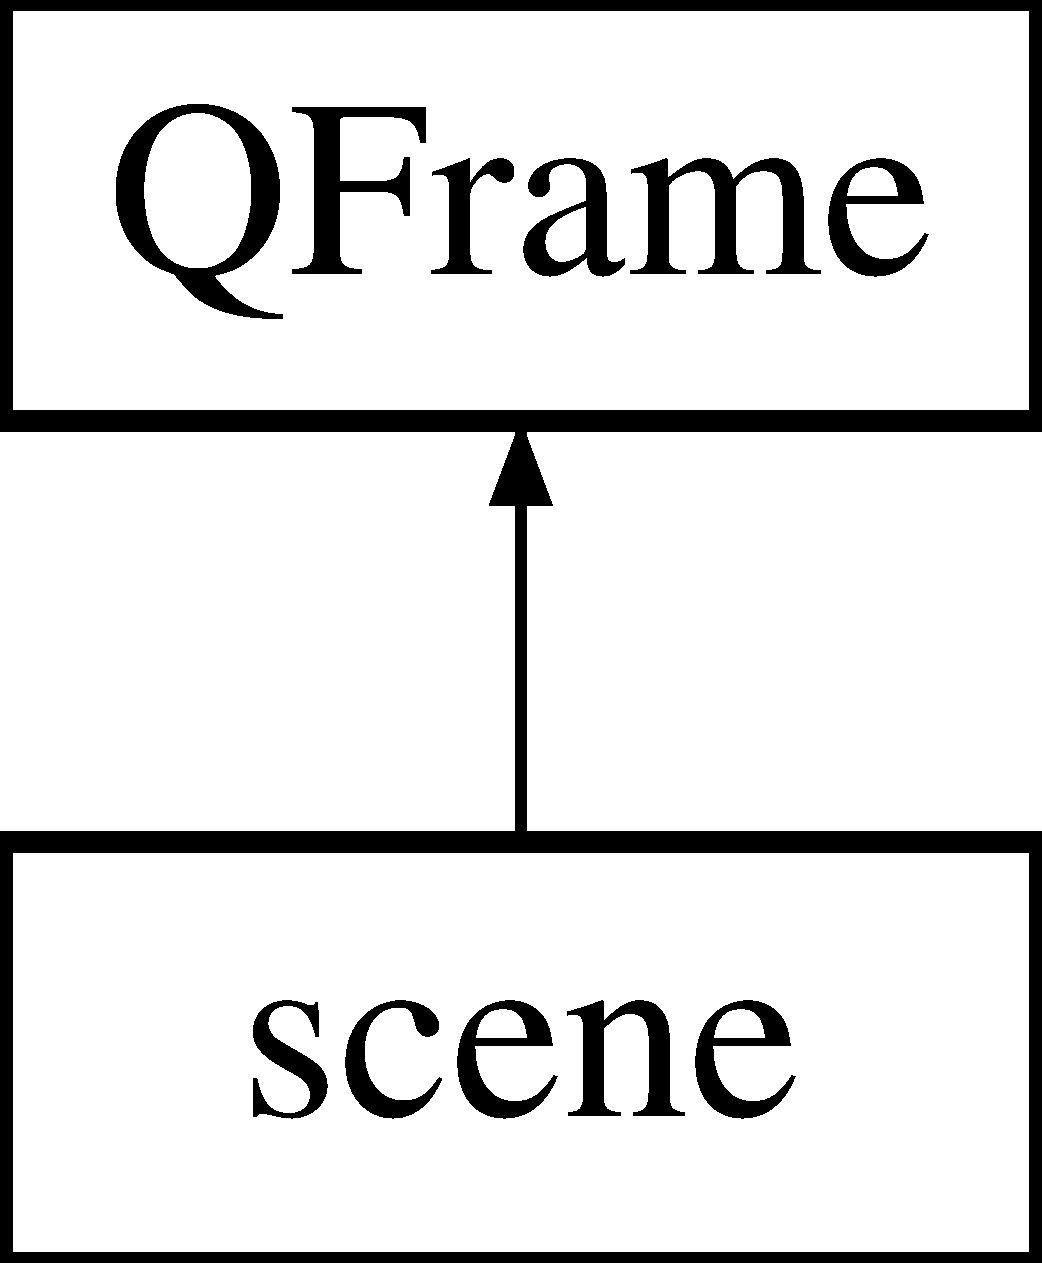
\includegraphics[height=2.000000cm]{classscene}
\end{center}
\end{figure}
\subsection*{Public Member Functions}
\begin{DoxyCompactItemize}
\item 
\mbox{\hyperlink{classscene_ac93fe52e7b2f23b16705b6cd79ab3d66}{scene}} (Q\+Widget $\ast$parent=0)
\begin{DoxyCompactList}\small\item\em Scene Constructor. \end{DoxyCompactList}\item 
Q\+Graphics\+Scene $\ast$ \mbox{\hyperlink{classscene_a89ba3baf41de3ed6dc530f606d083987}{get}} () const
\begin{DoxyCompactList}\small\item\em Scene getter. \end{DoxyCompactList}\end{DoxyCompactItemize}


\subsection{Constructor \& Destructor Documentation}
\mbox{\Hypertarget{classscene_ac93fe52e7b2f23b16705b6cd79ab3d66}\label{classscene_ac93fe52e7b2f23b16705b6cd79ab3d66}} 
\index{scene@{scene}!scene@{scene}}
\index{scene@{scene}!scene@{scene}}
\subsubsection{\texorpdfstring{scene()}{scene()}}
{\footnotesize\ttfamily scene\+::scene (\begin{DoxyParamCaption}\item[{Q\+Widget $\ast$}]{parent = {\ttfamily 0} }\end{DoxyParamCaption})\hspace{0.3cm}{\ttfamily [explicit]}}



Scene Constructor. 


\begin{DoxyParams}{Parameters}
{\em parent} & The parent to this current widget.\\
\hline
\end{DoxyParams}
continued description.... 

\subsection{Member Function Documentation}
\mbox{\Hypertarget{classscene_a89ba3baf41de3ed6dc530f606d083987}\label{classscene_a89ba3baf41de3ed6dc530f606d083987}} 
\index{scene@{scene}!get@{get}}
\index{get@{get}!scene@{scene}}
\subsubsection{\texorpdfstring{get()}{get()}}
{\footnotesize\ttfamily Q\+Graphics\+Scene $\ast$ scene\+::get (\begin{DoxyParamCaption}{ }\end{DoxyParamCaption}) const}



Scene getter. 

\begin{DoxyReturn}{Returns}
Scene object. 
\end{DoxyReturn}


The documentation for this class was generated from the following files\+:\begin{DoxyCompactItemize}
\item 
/\+Users/lukehutton/\+One\+Drive -\/ University of Leeds/\+University/\+Computer Science/\+Internship/moebinv-\/gui/include/scene.\+h\item 
/\+Users/lukehutton/\+One\+Drive -\/ University of Leeds/\+University/\+Computer Science/\+Internship/moebinv-\/gui/src/scene.\+cpp\end{DoxyCompactItemize}

%--- End generated contents ---

% Index
\backmatter
\newpage
\phantomsection
\clearemptydoublepage
\addcontentsline{toc}{chapter}{\indexname}
\printindex

\end{document}
